\documentclass{article} \usepackage{aaai} \usepackage{graphicx}

% Big margins for now so people can take notes/scribbles.
%\usepackage{fullpage}

\title{Parallel Best NBlock First}
\author{Ethan Burns \and Seth Lemons \and Wheeler Ruml \\
Department of Computer Science \\
University of New Hampshire \\
Durham, NH 03824 USA \\
\{eaburns,seth.lemons, ruml\}@unh.edu}
\date{\today}

\begin{document}
\maketitle

\begin{abstract}
We are approaching a time when it will no longer be beneficial for
hardware manufactures to create micro-processors with greater clock
speeds.  In order to get increased performance, software developers
will need to take advantage of concurrency and multi-core processors.
We propose a best-first-ish search algorithm which makes use of
multiple core CPUs in order to more quickly solve search problems
which are small enough to fit into memory.
\end{abstract}

\section{Introduction}

As microprocessor manufacturers build processors with more and more
cores, software developers are being pressured to create algorithms to
make better use of the newly available parallelism.

\section{Background}

\subsection{Structured Duplicate Detection}

In \cite{zhou:sdd} Zhou and Hansen propose a new method for external
memory graph search called Structured Duplicate Detection or SDD.  SDD
uses a projection function, which is a many-to-one mapping from states
in the search space to states in an abstract space, to decompose a
search graph.  The projection function creates an abstract space of
nodes that are projections, or images, of the nodes in the original
state space.  For a projection function $p$, $y$ is said to be the
\emph{image} of a node $x$ if $p(x) = y$.  Additionally $y'$ is a
successor of an abstract node $y$ if there are two states $x$ and $x'$
such that $x'$ is a successor of $x$, $y$ is the image of $x$ and $y'$
is the image of $x'$.  In other words:

\begin{eqnarray*}
&&x' \in successors(x) \wedge p(x) = y \wedge p(x') = y' \\
&\Rightarrow& y' \in successors(y)
\end{eqnarray*}

In the description of the SDD algorithm, the term \emph{nblock} is
used to refer to all nodes in the original state space that have the
same image in the abstract space, throughout the remainder of this
paper, the terms ``abstract state'', and ``nblock'' will be used
interchangeably since each nblock corresponds to a single abstract
state.

Zhou and Hansen show that, while performing duplicate detection, only
nodes within the same nblock must be checked for duplicates.  By the
definition of the successor set of an abstract node: any child node
$x'$ of a node $x$, in the original state space, will have an image
$p(x') \in successors(p(x))$, and therefore when performing duplicate
detection for $x'$ the only nodes that must be checked are in the
nblock $p(x') \in successors(p(x))$.  For this reason,
$successors(p(x))$ is called the \emph{duplicate detection scope} of
the nblock $p(x)$ -- no other nodes in the original state space will
ever need to be consulted for duplicate detection when expanding nodes
in the nblock $p(x)$.

This idea can be shown using the sliding tile puzzle as an example.
It is conceivable that a projection function for the sliding tiles
puzzle would be to only look at the position of the empty tile.  For
example: all states with the empty tile in the upper left-hand corner
(position 0) would map to the nblock shown in Figure
\ref{fig:tile-abstraction}, where the grayed square represents the
position of the empty tile.  Using this abstraction, there are sixteen
possible abstract states (one for each possible position of the empty
tile).  It is easy to see that all of the children of a state in the
nblock shown in this figure will have the empty tile in either
position 1 or 4 (either by sliding the tile in position 1 to the left,
or by sliding the tile in position 4 up).  Figure
\ref{fig:duplicate-detection-scope} shows the duplicate detection
scope for the nblock in Figure \ref{fig:tile-abstraction}.  Any of the
children of a state $x$ in the nblock shown in Figure
\ref{fig:tile-abstraction} will fall into one of the two nblocks shown
in Figure \ref{fig:duplicate-detection-scope}.

\begin{figure}[t]
\begin{center}
\includegraphics[width=1.5in]{images/tile-abstraction.eps}
\caption{The abstract image of all states with a empty tile in
  position 0.}
\label{fig:tile-abstraction}
\end{center}
\end{figure}

\begin{figure}[t]
\begin{center}
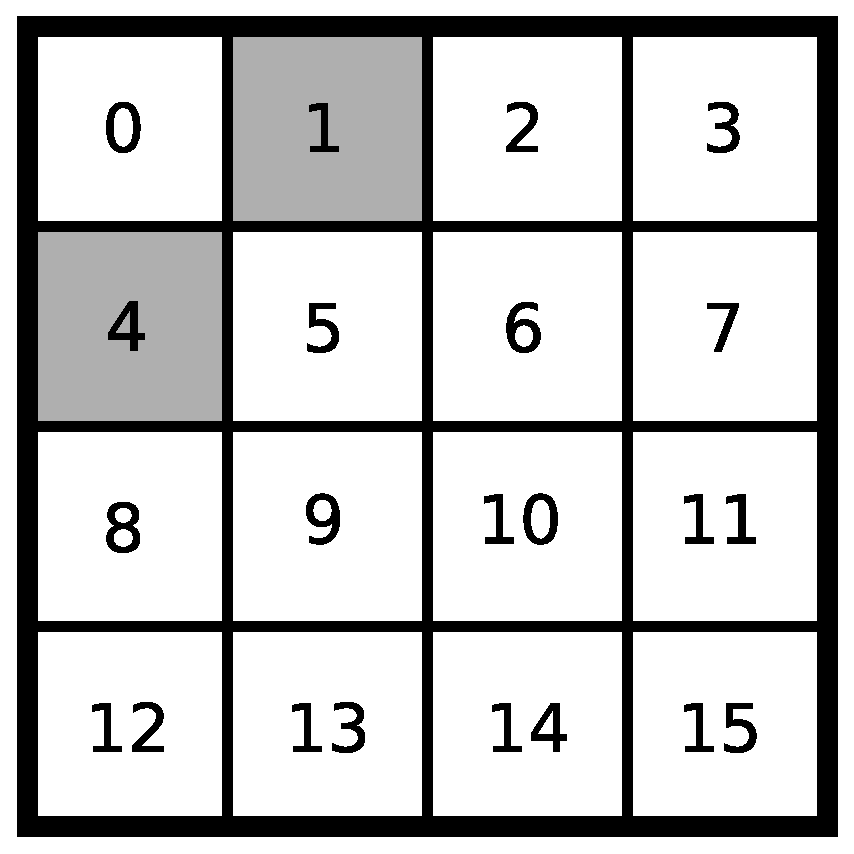
\includegraphics[width=1.5in]{images/duplicate-detection-scope.eps}
\caption{The duplicate detection scope of the abstract node shown in
  Figure \ref{fig:tile-abstraction}.}
\label{fig:duplicate-detection-scope}
\end{center}
\end{figure}

In \cite{zhou:sdd} Zhou and Hansen are interested in state space
decomposition so that they can explicitly move generated nodes to a
secondary storage device (such as a disk drive) when they are not
needed.  The SDD approach uses breadth-first heuristic search, where
one nblock is searched at a time.  Since duplicates can only fall into
the duplicate detection scope of the nblock being searched, the
remainder of the nodes can be pushed off to disk, instead of being
stored in main memory.  Nblocks can then be intelligently swapped into
and out of main-memory as the search progresses.

\subsection{Parallel Structured Duplicate Detection (PSDD)}

While the motivation of SDD is to have explicit control over which
portions of a search space reside in main-memory, Zhou and Hansen show
in \cite{zhou:psd} that this approach also lends itself to
parallelization.  The parallel SDD (or PSDD) algorithm uses the graph
of nblocks to find \emph{disjoint duplicate detection scopes}, or
duplicate detection scopes that do not overlap.  Nblocks with disjoint
duplicate detection scopes can be searched in parallel without any
locking or contention.  In order to find nblocks with disjoint
duplicate detection scopes the concept of a \emph{free} nblock is
introduced.  An nblock $b$ is considered to be free if no processor is
using an nblock in $successors(b)$ -- in other words, if all other
processors are searching nblocks with duplicate detection scopes which
are disjoint from that of $b$.  Free nblocks are found by tracking a
$\sigma(b)$ value for each nblock $b$, where $\sigma(b)$ is the number
of nblocks in $successors(b)$ that are in use by another processor.
Any nblock $b$ with $\sigma(b) = 0$ is free, and therefore a processor
can acquire $b$ and its duplicate detection scope for a period of lock
free expansion.  PSDD is an attractive algorithm because it only uses
a single shared data structure (the nblock graph) which reduces the
amount of contention between processors during a search.

In PSDD, as in SDD, the search progresses in layers, in a
breadth-first manor.  For example, an nblock can be thought of as a
closed-list and two open-lists -- one open-list for the current layer
(which is being expanded from) and one for the next layer (which is
being expanded into).  Nodes are removed from the open-list of the
current layer of an nblock, duplicate detection is performed from the
closed-list, if the node is not a duplicate its children are inserted
into the next layer open-list for their respective nblocks.  When the
current layer for an nblock is done expanding, it is added to the free
nblock list for the next layer, and the processor tries to acquire a
new free nblock in the current layer.  Once there are no more nblocks
to expand on the current layer, the search switches to the next layer
and begins again.  The search progresses in this fashion until a goal
is found or the entire search space is covered and there is no
solution.  Since the search order is breadth-first, the first goal
that is found is the optimal goal.

\section{Parallel Best NBlock First (PBNF)}
\subsection{Safe PBNF}
\section{Experimental Results}
\section{Conclusion}

\bibliography{master}
\bibliographystyle{aaai}

\end{document}
